\documentclass[12pt]{article}
\everymath{\displaystyle}
\usepackage{unicode-math}
\usepackage{pgfplots}
\pgfplotsset{compat=1.18}
\usepackage{amsmath}



\usepackage[margin=1in]{geometry}
\usepackage{tcolorbox}
\usepackage{graphicx}
\usepackage{tikz}
\usepackage{amssymb}
\usepackage{enumitem}
\usepackage{titlesec}
\usepackage{fancyhdr}
\usepackage{pifont}
\usepackage{xcolor}
\newcounter{questionnum}
\setcounter{questionnum}{0}
\usepackage{eso-pic} % for page background

% --------- 主题颜色设置 ---------
\definecolor{novelblue}{RGB}{70,60,150}
\definecolor{headerbg}{RGB}{240,240,255}

\pagestyle{fancy}
\fancyhf{}
\renewcommand{\headrulewidth}{0.4pt}
\renewcommand{\headrule}{\hbox to\headwidth{\color{novelblue}\leaders\hrule height 0.4pt\hfill}}

% --------- 页眉背景色条 ---------
\newcommand{\headbackground}{
  \AddToShipoutPictureBG*{
    \begin{tikzpicture}[remember picture, overlay]
      \fill[blue!5!purple!10] (current page.north west) rectangle ([yshift=-60pt]current page.north east);
    \end{tikzpicture}
  }
}

% --------- 页眉设置 ---------
\pagestyle{fancy}
\fancyhf{}
\renewcommand{\headrulewidth}{0pt}
\fancyhead[L]{\color{novelblue}\textbf{\textbf{Novel Prep} }}
\fancyhead[C]{\color{novelblue}\textbf {SAT Preparation}}
\fancyhead[R]{\color{novelblue}\textbf{Jack Zeng}}


\newtcolorbox{SATCard}[1][]{%
  enhanced,
  colback=white,
  colframe=novelblue,
  coltitle=white,
  boxrule=0.6pt,
  arc=4pt,
  boxsep=5pt,
  left=8pt, right=8pt, top=10pt, bottom=10pt,
  sharp corners=south,
  drop shadow south east,
  #1
}

% --------- 顶部 Mark for Review 栏 ---------
\newcommand{\markforreview}{
  \stepcounter{questionnum} % 自动递增题号
  \begin{tikzpicture}[scale=1.1]
    % 黑色题号
    \fill[black] (0,0) rectangle (0.8,0.6);
    \node[white, font=\bfseries\large] at (0.4,0.3) {\thequestionnum};

    % 灰底主栏
    \fill[gray!10] (0.8,0) rectangle (14.5,0.6);

    % Mark for Review
    \node[anchor=west, font=\small] at (1.2,0.3) {\ding{72} \hspace{2pt}Mark for Review};

    % ABC 按钮区域
    \draw[thick, rounded corners=3pt] (13.5,0.12) rectangle (14.5,0.48);
    \node[font=\bfseries\normalsize] at (14.0,0.3) {ABC};
  \end{tikzpicture}


  \newcommand{\choiceboxcircled}[2]{%
  \begin{tcolorbox}[
    colback=white,
    colframe=black,
    boxrule=0.5pt,
    rounded corners=6pt,
    left=6pt, right=6pt, top=6pt, bottom=6pt,
    width=\linewidth
  ]
    \textbf{\large\textcircled{\textbf{#1}}} \ #2
  \end{tcolorbox}
}
}

% --------- 选项框样式 ---------
\newcommand{\choicebox}[2]{%
  \begin{tcolorbox}[
    colback=white, 
    colframe=novelblue,
    boxrule=0.5pt, 
    rounded corners=4pt, 
    left=6pt, right=6pt, top=6pt, bottom=6pt,
    width=\linewidth
  ]
  \textbf{#1.} \ #2
  \end{tcolorbox}
}


\begin{document}
\section*{Math Hard Question 10}

\noindent\markforreview
\vspace{1em}

\begin{center}
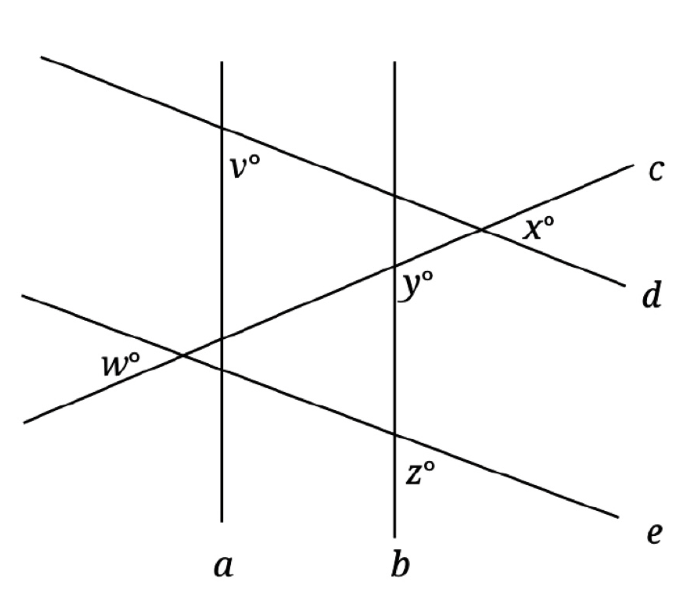
\includegraphics[width=0.4\textwidth]{f8.png}
\end{center}

In the figure, parallel lines \(a\) and \(b\) are intersected by lines \(c\), \(d\), and \(e\).  
If \(z = 49^\circ\), \(y = 136^\circ\), and \(v < z\), which statement about \(x\) and \(w\) must be true?

\choicebox{A}{\(x < w\)}  
\choicebox{B}{\(x > w\)}  
\choicebox{C}{\(x = w\)}  
\choicebox{D}{\(x + w = 90\)}

\vspace{2em}

\newpage
\noindent\markforreview
\vspace{1em}

The functions \(f\) and \(g\) are defined by the given equations below, where \(x \geq 0\).  
Which of the following equations displays, as a constant or coefficient, the minimum value of the function it defines?

\begin{itemize}
\item[I.] \(f(x) = 16(1.3)^{x+5}\)
\item[II.] \(g(x) = 16(1.09)(1.3)^{x+3}\)
\end{itemize}

\choicebox{A}{I only}  
\choicebox{B}{II only}  
\choicebox{C}{I and II}  
\choicebox{D}{Neither I nor II}

\vspace{2em}

\noindent\markforreview
\vspace{1em}

The table shows values of \(x\) and corresponding values of \(g(x)\), where:  
\[
g(x) = \frac{f(x)}{x + 3}
\]  
and \(f(x)\) is a linear function.  

What is the \(y\)-intercept of the graph of \(y = f(x)\) in the \(xy\)-plane?

\[
\begin{array}{c|c}
x & g(x) \\
\hline
-15 & 3 \\
-6 & 0 \\
9 & 5 \\
\end{array}
\]

\choicebox{A}{(0, -6)}  
\choicebox{B}{(0, 4)}  
\choicebox{C}{(0, 8)}  
\choicebox{D}{(0, 24)}

\vspace{2em}

\noindent\markforreview
\vspace{1em}

The positive number \(a\) is 2,106\% of the sum of the positive numbers \(b\) and \(c\),  
and \(b\) is 81\% of \(c\).  

What percent of \(b\) is \(a\)?

\choicebox{A}{4706\%}  
\choicebox{B}{2600\%}  
\choicebox{C}{38.12\%}  
\choicebox{D}{21.87\%}

\vspace{2em}
\noindent\markforreview
\vspace{1em}

In the given equation, \(u\) is a positive constant.  
The sum of the solutions to the equation is 1. What is the value of \(u\)?  
\[
7x^2(3x - 11)(3x - u) = 0
\]

\choicebox{A}{1}  
\choicebox{B}{-8}  
\choicebox{C}{\(\frac{11}{3}\)}  
\choicebox{D}{\(\frac{8}{3}\)}

\vspace{2em}

\newpage
\noindent\markforreview
\vspace{1em}

Which of the following values of \(x\) satisfy the equation  
\[
-3x^2 + 12x + 4 = 0
\]

\choicebox{A}{0}  
\choicebox{B}{\(-2\) and 2}  
\choicebox{C}{\(2 - \frac{2\sqrt{6}}{3}\) and \(2 + \frac{2\sqrt{6}}{3}\)}  
\choicebox{D}{\(2 - \frac{4\sqrt{3}}{3}\) and \(2 + \frac{4\sqrt{3}}{3}\)}

\vspace{2em}

\noindent\markforreview
\vspace{1em}

A line intersects two parallel lines, forming four acute angles and four obtuse angles.  
The measure of one of these eight angles is \((7x - 250)^\circ\).  
The sum of the measures of four of the eight angles is \(k\).  

Which of the following could **not** be equivalent to \(k\) for all values of \(x\)?

\choicebox{A}{\(-14x + 1540\)}  
\choicebox{B}{\(14x - 320\)}  
\choicebox{C}{\(-28x + 1720\)}  
\choicebox{D}{360}

\newpage
\noindent\markforreview
\vspace{1em}

The triangle inequality theorem states that the sum of any two sides of a triangle  
must be greater than the length of the third side.  

If a triangle has side lengths of 7 and 10,  
which inequality represents the possible lengths, \(x\), of the third side of the triangle?

\choicebox{A}{\(x < 17\)}  
\choicebox{B}{\(x > 17\)}  
\choicebox{C}{\(3 < x < 17\)}  
\choicebox{D}{\(x < 3\) or \(x > 17\)}

\vspace{2em}








\end{document}